\documentclass{article}

\usepackage[italian]{babel}
\usepackage[T1]{fontenc}
\usepackage[utf8]{inputenc}
\usepackage[pageanchor]{hyperref}
\hypersetup{
	colorlinks=true,
	linkcolor=blue
	}
\usepackage{graphicx}
\def\code#1{\texttt{#1}}

\title{{\huge AuleLibere: un visualizzatore dello stato di occupazione delle aule dipartimentali}}
\author{Arianna Masciolini, matricola 285025\\ Tommaso Ricci, matricola 287123}
\date{A.A. 2016-2017}


\begin{document}
	\maketitle
	\newpage
	\tableofcontents
	\newpage
	\part{Introduzione al progetto}
	\section{Abstract}
	Rivolta principalmente agli studenti che utilizzano le aule per la didattica frontale anche per lo studio di gruppo, l'applicazione permette di individuare le aule libere del Dipartimento di Matematica ed Informatica dell'Università degli Studi di Perugia grazie ad una semplice interfaccia grafica in cui le informazioni sono visualizzate sulle planimetrie dell'edificio.
	\section{Obiettivi}
	Obiettivo principale del progetto è, pertanto, fornire agli utenti un'alternativa rapida ed efficace alla consultazione del tabellone orario. Lo studente avrà in tasca le informazioni essenziali, da consultare agevolmente anche in mobilità quando gli fosse utile conoscere in anticipo la situazione.
	\paragraph{Prospettive e sviluppi futuri}
	Nelle versioni successive, ci si propone di aggiungere svariate funzionalità all'applicativo; innanzitutto la possibilità, per gli utenti, di comunicare informazioni sullo stato delle aule in tempo reale, in modo da rendere più accurati e completi i dati visualizzati. In tale scenario, ci si propone inoltre di tracciare, con lo stesso sistema, lo stato di occupazione dei tavoli collocati nei vari pianerottoli. Obiettivo a lungo termine, infine, è quello di creare una procedura per la creazione di mappe, così da facilitare la diffusione di questo sistema in contesti esterni a quello del DMI.
	\newpage
	\part{Documento di analisi}
	\section{Analisi dei requisiti e descrizione delle soluzioni adottate} 
	La decisione di realizzare un applicativo Android si deve alla sua grande diffusione nel mondo dei dispositivi mobili, al quale il progetto si rivolge.
	Occorre innanzitutto che l'applicazione, dalle funzionalità volutamente minimali, recuperi i dati relativi alla gestione delle aule dipartimentali dalle fonti ufficiali. Una prima possibilità per ottenere quanto descritto è il web scraping: i dati sono infatti pubblicati in una pagina del sito web del Dipartimento, che offre ai visitatori un servizio in parte analogo a quello che l'applicazione si propone di adattare alle esigenze degli studenti, rivolto però principalmente agli insegnanti, che autenticandosi possono prenotare le aule. A questa strategia si è preferita però l'interrogazione diretta del database mySQL che contiene in forma più completa e maneggevole le informazioni relative alle prenotazioni delle aule dipartimentali: il database \textbf{mrbs}. Le query vengono effettuate tramite un sistema di chiamate API: allo stato attuale, al fine di testare l'applicazione con dati reali, si sta utilizzando una copia del database sopra citato aggiornata al 13/07/2017, hostata in un'istanza AWS EC2 consistente in un server Apache.
	Per quel che riguarda l'interfaccia utente, sono di massima importanza leggibilità e facilità d'uso. Si è scelto pertanto di utilizzare, ripulite da ogni dettaglio superfluo, le planimetrie del DMI, utilizzando un color coding intuitivo per descrivere, tramite immagini in sovraimpressione, lo stato delle diverse classi. Viste le dimensioni limitate degli schermi degli smartphone, ogni schermata mostra un solo piano dell'edificio: vi è dunque una sola \code{Activity} principale, suddivisa in tanti frammenti quanti sono i piani del DMI, accessibili tramite un semplice swipe. Infine, grazie ad un sistema mappatura delle planimetrie, al tocco della superficie di un'aula l'utente potrà visualizzare alcune informazioni aggiuntive riguardo il suo utilizzo o, nel caso di laboratori e biblioteche, gli orari di apertura e chiusura.
	\paragraph{Metodologie di sviluppo}
	La metodologia adottata per lo sviluppo dell'app Android si basa sull'approccio incrementale, più efficiente e gratificante rispetto al tradizionale modello a cascata, specialmente per sviluppatori alle prime armi. Per ragioni analoghe, si è deciso di coniugare i rilasci successivi con l'idea di pair programming.
	Al fine di semplificare la collaborazione tra i due autori del progetto quando non si è rivelato possibile lavorare alla stessa postazione e per facilitare, in futuro, la diffusione e il miglioramento dell'applicazione, si è deciso di pubblicarne il codice sorgente, disponibile all'indirizzo \url{https://github.com/Disorganizzazione/AuleLibere}.
	L'ambiente di programmazione utilizzato è Android Studio.
	\section{Requisiti minimi di sistema}
	Sistema operativo Android 4.2.2 (Jelly Bean) o superiore, 1 GB RAM, processore single-core 1 Ghz, accesso ad internet.
	\newpage
	\part{Documentazione UML}
	\section{Diagramma di classe}
	Nel diagramma di classe, per chiarezza, si è scelto di inserire,  lasciandole vuote, anche le classi estese e le interfacce implementate direttamente preesistenti il progetto. Anche la classe Maps, creata automaticamente da Android Studio, è stata lasciata vuota, in modo da rendere il diagramma il più possibile esplicativo del lavoro svolto.
	\begin{figure}[h]
		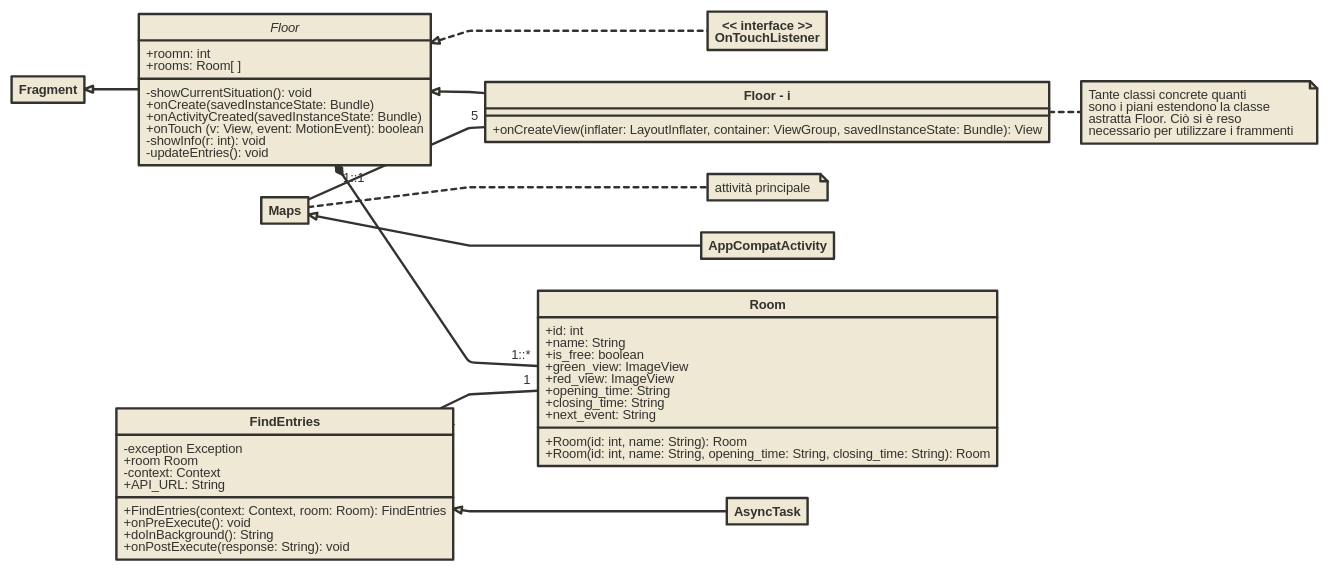
\includegraphics[width=\textwidth]{class}
		\centering
		\caption{Diagramma delle classi}
	\end{figure}
	\newpage
	\section{Casi d'uso}
	Nel diagramma dei casi d'uso si sono volute lasciare, per completezza, anche indicazioni sulle azioni che l'utente potrà compiere nelle versioni future dell'applicazione.\\\\
	\begin{figure}[h]
		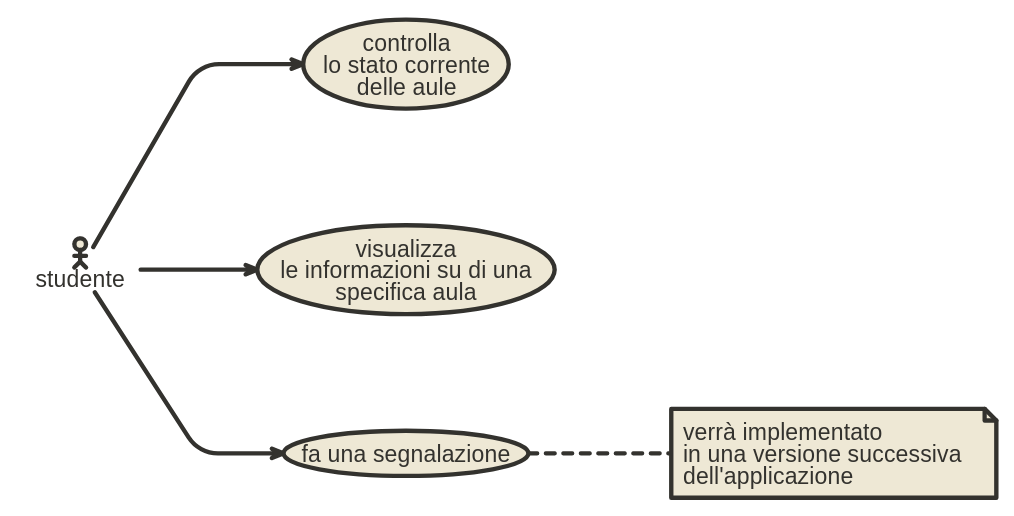
\includegraphics[width=\textwidth]{casiduso}
		\centering
		\caption{Diagramma dei casi d'uso}
	\end{figure}
	\newpage
	\section{Diagramma di sequenza}
	\begin{figure}[h]
		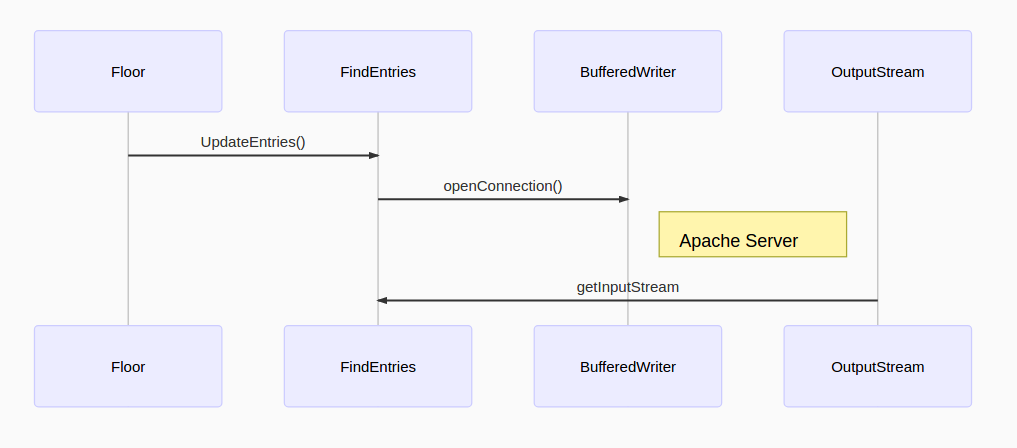
\includegraphics[width=\textwidth]{seq}
		\centering
		\caption{Diagramma di sequenza}
	\end{figure}
	\newpage
	\section{Diagramma di stato}
	Lo stato di un'aula varia in modo ciclico: solo per rispettare le convenzioni, si è comunque scelto come stato iniziale quello in cui l'aula è chiusa; tuttavia la scelta è del tutto arbitraria, per cui si è rinunciato a definire anche uno stato finale distinto, dal momento che tale decisione avrebbe costituito una forzatura.\\\\
	\begin{figure}[h]
		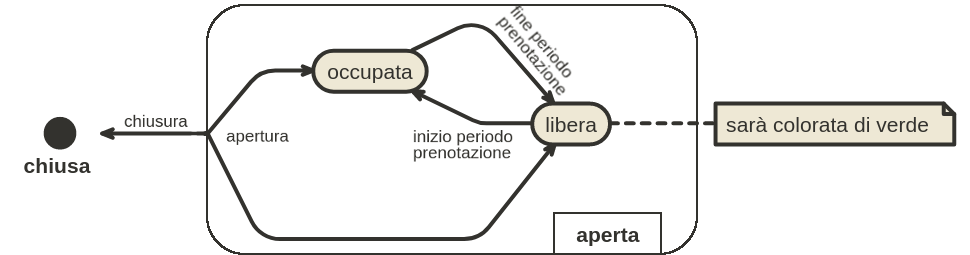
\includegraphics[width=\textwidth]{stato}
		\centering
		\caption{Diagramma di stato relativo ad un'aula}
	\end{figure}
	\newpage
	\section{Diagramma di attività}
	Il diagramma di attività offre una descrizione esaustiva delle principali interazioni con l'applicazione attualmente possibili per l'utente.\\\\
	\begin{figure}[h]
		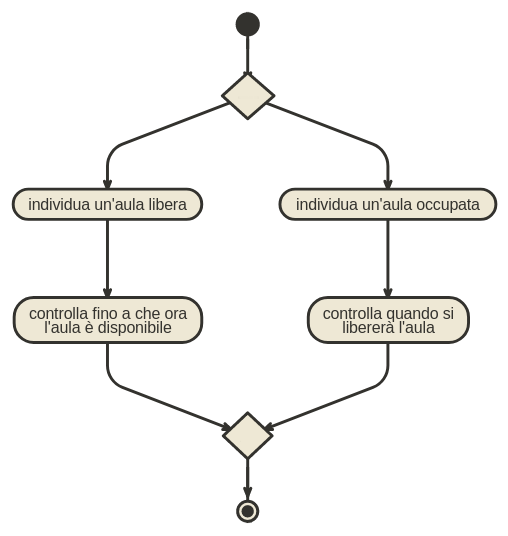
\includegraphics[width=\textwidth]{attivita}
		\centering
		\caption{Diagramma di attività}
	\end{figure}
	\newpage
	\part{Test funzionali}
	Particolarmente interessante testare non tanto le vere e proprie interazioni tra utente ed applicazione, che si limitano allo swipe per le transizioni da un frammento a un altro e al tocco di un'aula per la visualizzazione di informazioni aggiuntive, quanto il comportamento dell'applicazione al variare dell'ora e del giorno della settimana. Il programma utilizza in diversi modi la data e l'ora impostate sul telefonino: per determinare se l'università è aperta o chiusa, per decidere se una specifica aula è aperta o chiusa secondo il suo orario -si pensi ad esempio ai laboratori, che hanno un orario differente rispetto a quello degli altri ambienti-, per determinare, in base al risultato delle query, se le aule sono libere od occupate e, soprattutto, per effettuare la query che determina quali aule siano occupate in un dato momento. Indirettamente, in ogni caso, si possono interpretare data ed ora correnti come un input da parte dell'utente (che, peraltro, può effettivamente impostarle a suo piacimento). Potrebbe sembrare, dal momento che una data altro non è che un numero intero positivo (secondi trascorsi dal 1/1/1970) che tutti gli input siano validi. Osserviamo subito però che, per il formato impiegato nel database per indicare i momenti di inizio e fine di una prenotazione (Unix Timestamp) gli input ammissibili sono limitati sia superiormente che inferiormente.
	Un possibile set di casi di test funzionali è dunque:\\
	
\begin{table}[h]
	\centering
	\label{my-label}
	\begin{tabular}{|l|l|l|}
		\hline
		n. & Time       & Validità \\ \hline
		1  & 1501448305 & V        \\ \hline
		2  & -1         & NV       \\ \hline
		3  & 4294967296 & NV       \\ \hline
	\end{tabular}
	
\end{table}

Dove abbiamo come casi estremi:

\begin{table}[h]
	\centering
	\label{my-label}
	\begin{tabular}{|l|l|}
		\hline
		Validi        & Non validi     \\ \hline
		0, 2147483647 & -1, 2147483648 \\ \hline
	\end{tabular}
\end{table}

	\newpage
	\part{Design pattern} %(Siamo sicuri?)
	Un pattern creazionale che ben si adatta alla situazione presentata, e che si terrà in cosiderazione per sviluppi futuri, è l' \textbf{Abstract Factory o Kit}, che consente di rendere intercambiabili diverse implementazioni che soddisfano una determinata interfaccia. E' questo il caso delle molteplici classi che estendono \code{Floor} (si veda a tal proposito il diagramma delle classi a \hyperlink{page.5}{pag. 5}), tanto simili fra loro che le si sarebbe volute implementare come un' unica classe \code{Floor}, provvista di un costruttore con parametri volti ad attribuire ad ogni piano le proprie caratteristiche specifiche (ad esempio, le aule in esso situate). Tuttavia, per l'uso che se ne fa, \code{Floor} deve necessariamente essere una sottoclasse di \code{Fragment}, il che impedisce l'uso di costruttori differenti da quello di default. Per il momento, difatti, si è deciso semplicemente di rendere \code{Floor} una classe astratta ed estenderla per ogni piano del Dipartimento.
	\newpage
	\appendix
	\part{Glossario}
	\textit{\textbf{Aula dipartimentale}}: aula situata all'interno del dipartimento, aperta agli studenti almeno in alcuni orari. Si considerano aule dipartimentali le aule per la didattica frontale, le biblioteche, i laboratori e le aule studio, \textbf{non} sono compresi nella definizione gli uffici dei docenti e del personale tecnico amministrativo. Nel codice, ogni aula dipartimentale è un'istanza della classe \code{Room}.\\\\
	\textit{\textbf{Piano}}: nel contesto dell'applicazione, quando si parla di "piano" si fa riferimento alla classe \code{Floor}, utilizzata per descrivere i veri e propri piani del dipartimento tramite la loro caratteristica saliente: un \code{Floor} è, difatti, un array di \code{Room}, cui corrisponde un layout xml costituito da più immagini in sovrapposizione.\\\\
	\textit{\textbf{Database mrbs}}: database contenente tutte le informazioni relative alle aule dipartimentali e al loro utilizzo.\\\\
	\textit{\textbf{Frammento}}: Porzione della UI in un'\code{Activity} di un'applicazione Android. Il termine "frammento" fa riferimento alla classe \code{Fragment} delle librerie Java per Android; che nel progetto è utilizzata tramite la classe \code{Floor}, che la estende.\\\\
	\textit{\textbf{AWS (Amazon Web Services)}}: Cloud provider.\\\\
	\textit{\textbf{EC2 (Elastic Cloud Computing)}}: Servizio cloud impiegato nel progetto per la creazione del server e la gestione del database.
	%(Segue)
\end{document}
